\section{Tutorial: ¿Dónde está Mi Auto?}

Te estacionaste lo más cerca posible al estadio, pero cuando el
concierto termina, no recuerdas dónde está tu auto! Tus amigos tampoco
se acuerdan...

Afortunadamente, no has perdido tu teléfono Android, él nunca olvida
nada :-)!!

Además recuerdas que tiene la excelente aplicación \appName{¿Dónde está mi
Auto?}. Con esta aplicación, presionas un botón cuando el auto, y el teléfono utiliza el sensor de ubicación para registrar las
coordenadas GPS y dirección del auto. Más tarde, al reabrir la
aplicación, te da indicaciones sobre cómo llegar a tu auto desde tu
ubicación actual!

\subsection*{Qué Aprenderás}

Esta aplicación abarca los siguientes conceptos:

\begin{itemize}

\item Determinar la ubicación del dispositivo Android utilizando el
  componente \component{SensorDeUbicación}.

\item Registrar datos en una base de datos directamente en el equipo
  utilizando \component{TinyDB}.

\item Utilizar el componente \component{ActivityStarter} para abrir
  Google Maps desde tu aplicación y mostrar indicaciones para llegar a
  una dirección desde la ubicación actual.
\end{itemize}

\subsection*{Diseñar los Componentes}

La interfaz de usuario de \appName{¿Dónde está mi Auto?} consiste en
etiquetas para mostrar tu ubicación actual y las ubicaciones
recordadas, y botones para registrar una ubicación y mostrar
indicaciones para llegar hacia esta ubicación. Necesitarás etiquetas
que muestran texto estático; por ejemplo, \component{EtiquetaGPS}
mostrará el texto ``GPS:'' que aparece en la interfaz usuario. Otras
etiquetas, como \component{EtiquetaLatActual}, mostrarán datos del
sensor de ubicación (en este caso la latitud). Para estas etiquetas,
pondrás un valor por defecto, (0,0), que cambiará con la adquisición
de nueva información de ubicación por el GPS.

También necesitarás tres componentes invisibles:
\component{SensorDeUbicación} para obtener la ubicación actual,
\component{TinyDB} para almacenar ubicaciones persistentemente, y
\component{ActivityStarter} para lanzar Google Maps para obtener
indicaciones desde la ubicación actual hacia la ubicación almacenada.

Puedes construir la interfaz de usuario basándote en
la~\Cref{fig:Sensors1}.

\begin{figure}[H]
\vspace{3em}
\centering
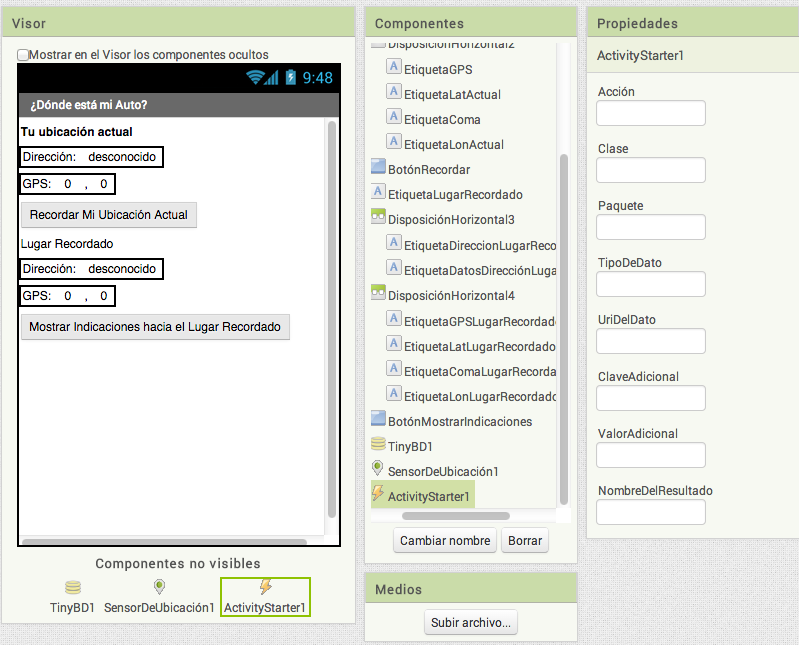
\includegraphics[scale=0.3]{Sensors1}
\caption{La aplicación \appName{¿Dónde está mi Auto?} en el \componentDesigner.}
\label{fig:Sensors1}
\end{figure}

Puedes construir la interfaz de usuario mostrada en
la~\Cref{fig:Sensors1} utilizando los componentes que se muestran en
la Tabla~\ref{tab:Sensors1}.

\begin{table}
\begin{footnotesize}
\begin{tabular}{|l|l|p{6cm}|}
\hline
Tipo de Componente & Nombre & Propósito\\\hline

\component{Etiqueta} &
EtiquetaUbicaciónActual &
Muestra el texto ``Tu ubicación actual''
\\\hline

\component{DisposiciónHorizontal} &
DisposiciónHorizontal1 &
Ordena la información sobre la dirección actual
\\\hline

\component{Etiqueta} &
EtiquetaDirecciónActual &
Muestra el texto ``Dirección:''
\\\hline

\component{Etiqueta} &
EtiquetaDatosDirecciónActual &
Muestra información dinámica: la dirección actual.
\\\hline

\component{DisposiciónHorizontal} &
DisposiciónHorizontal2 &
Ordena la información del GPS.
\\\hline

\component{Etiqueta} &
EtiquetaGPS &
Muestra el texto ``GPS:''.
\\\hline

\component{Etiqueta} &
EtiquetaLatActual &
Muestra información dinámica: la latitud actual.
\\\hline

\component{Etiqueta} &
EtiquetaComa &
Muestra el texto ``,''.
\\\hline

\component{Etiqueta} &
EtiquetaLonActual &
Muestra información dinámica: la longitud actual.
\\\hline

\component{Botón} &
BotónRecordar &
Presionar para almacenar la ubicación actual.
\\\hline

\component{Etiqueta} &
EtiquetaLugarRecordado &
Muestra el texto ``Lugar Recordado''.
\\\hline

\component{DisposiciónHorizontal} &
DisposiciónHorizontal3 &
Ordena la información sobre el lugar recordado.
\\\hline

\component{Etiqueta} &
EtiquetaDirecciónLugarRecordado &
Muestra el texto: ``Dirección''.
\\\hline

\component{Etiqueta} &
EtiquetaDatosDirecciónLugarRecordado &
Muestra información dinámica: la dirección del lugar recordado.
\\\hline

\component{DisposiciónHorizontal} &
DisposiciónHorizontal4 &
Ordena la informacion sobre el GPS del lugar recordado.
\\\hline

\component{Etiqueta} &
EtiquetaGPSLugarRecordado &
Muestra el texto ``GPS:''.
\\\hline

\component{Etiqueta} &
EtiquetaLatLugarRecordado &
Muestra información dinámica: la latitud del lugar recordado.
\\\hline

\component{Etiqueta} &
EtiquetaComa2 &
Muestra el texto ``,''.
\\\hline

\component{Etiqueta} &
EtiquetaLatActual &
Muestra información dinámica: la longitud del lugar recordado.
\\\hline

\component{Botón} &
BotónMostrarIndicaciones &
Presionar para obtener indicaciones desde la ubicación actual hacia el
lugar recordado.
\\\hline

\component{SensorDeUbicación} &
SensorDeUbicación1 &
Siente la información del GPS.
\\\hline

\component{TinyDB} &
TinyDB1 &
Almacena el lugar recordado de manera persistente.
\\\hline

\component{VisorWeb} &
VisorWeb1 &
Muestra las indicaciones desde la ubicación actual hacia el lugar recordado.
\\\hline

\end{tabular}
\end{footnotesize}
\caption{Todos los componentes para la aplicación.}
\label{tab:Sensors1}
\end{table}

Configura los componentes de la Tabla~\ref{tab:Sensors1} de la
siguiente manera:

\begin{itemize}
\item Ajusta la propiedad \property{Texto} de las etiquetas con
  algunos textos fijos (``Dirección:'', ``GPS'', ``,'').
\item Ajusta la propiedad \property{Texto} de los datos dinámicos del
  GPS como ``0,0''.
\item Ajusta la propieda \property{Texto} de las direcciones dinámicas
  como ``desconocido''.
\item Desactiva la propiedad \property{Habilitado} de los botones
  \component{BotónRecordar} y \component{BotónMostrarIndicaciones}.
\item Desactiva la propiedad \property{Enrollable} del component
  \component{Screen1}. Así, el \component{VisorWeb} cabrá en la
  pantalla.
\end{itemize}

\begin{table}
\centering
\begin{footnotesize}
\begin{tabular}{|l|p{7cm}|}
\hline
Propiedad & Valor \\\hline
Acción & android.intent.action.VIEW \\\hline
Clase & com.google.android.maps.MapsActivity \\\hline
Paquete & com.google.android.apps.maps \\\hline
\end{tabular}
\end{footnotesize}
\caption{Propiedades de \component{ActivityStarter} para lanzar Google Maps.}
\label{tab:Sensors2}
\end{table}

\paragraph{Nota} El componente \component{ActivityStarter} deja que la
aplicación abra cualquier aplicación Android instalada en el
dispositivo. Las propiedades listadas en la Tabla~\ref{tab:Sensors2}
deben ser utilizadas textualmente para abrir Maps; para abrir otros
mapas o aplicaciones, ver la documentación de App Inventor en
\url{http://ai2.appinventor.mit.edu/reference/components/connectivity.html#ActivityStarter}.

\subsection*{Añadir comportamientos a los componentes}

{Necesitarás los comportamientos siguientes para la aplicación:}

\begin{itemize}
\item Cuando el \component{SensorDeUbicación} tiene una lectura,
  coloca los datos de la ubicación actual en las etiquetas apropiadas
  de la interfaz de usuario. De esta manera, el usuario sabrá que el
  sensor ha leído una ubicación y que está listo para guardarla.

\item Cuando el usuario presiona el \component{BotónRecordar}, copia
  los datos de la ubicación actual en las etiquetas hacia la ubicación
  a recordar.También necesitarás almacenar los datos de la ubicación a
  recordar para que estén guardados de forma persistente si el usuario
  cierra y vuelve a abrir la aplicación.

\item Cuando el usuario presiona el
  \component{BotónMostrarIndicaciones}, abre la aplicación Google Maps
  para que muestre indicaciones para llegar a la ubicación almacenada.

\item Cuando la aplicación sea abierta nuevamente, carga la ubicación
  almacenada desde la base de datos dentro de la base de datos.
\end{itemize}

\subsubsection*{Mostrar la ubicación actual}

El evento \block{SensorDeUbicación.CambioEnUbicación} ocurre no sólo cuando la
ubicación del equipo cambia, sino que también cuando el sensor tiene
su primera lectura.

A veces, esta primera lectura puede demorar algunos segundos, y a
veces no tendrás ninguna lectura si no hay conexión con los satélites
GPS (y dependendiendo de los ajustes del equipo).

Cuando tienes una lectura de ubicación, la aplicación debería colocar
los datos en las etiquetas apropiadas. La Tabla~\ref{tab:Sensors3}
muestra todos los bloques que necesitarás para realizar esto.

\begin{table}
\centering
\begin{footnotesize}
\begin{tabular}{|l|p{6cm}|}
\hline
Tipo de Bloque & Propósito\\\hline

\block{SensorDeUbicación1.CambioDeUbicación} &
Es el controlador de evento que se activa cuando el teléfono recibe
una nueva lectura GPS.\\\hline

\block{poner EtiquetaDatosDirecciónActual.Texto} &
Coloca los datos nuevos en la etiqueta para la dirección
actual.\\\hline

\block{SensorDeUbicación.DirecciónActual} &
Esta propiedad te da la dirección ``de calle'' asociada a la última
lectura del GPS.\\\hline

\block{poner EtiquetaLatActual.Texto} & Coloca la latitud actual en la
etiqueta correspondiente.\\\hline

Valor \parameter{latitud} & Se conecta en el bloque \block{poner
  EtiquetaLatActual.Texto}.\\\hline

\block{poner EtiquetaLonActual.Texto} & Coloca la longitud actual en
la etiqueta correspondiente.\\\hline

Valor \parameter{longitud} & Se conecta en el bloque \block{poner
  EtiquetaLonActual.Texto}.\\\hline

\block{poner BotónRecordar.Habilitado} & Activa el botón para
registrar la lectura de la ubicación actual.\\\hline

Bloque lógico \block{cierto} & Se conecta en el bloque \block{poner BotónRecordar.Habilitado}\\\hline
\end{tabular}
\end{footnotesize}
\caption{Bloques para obtener una lectura de ubicación y mostrarla en
  la interfaz de usuario de la aplicación.}
\label{tab:Sensors3}
\end{table}

Como se muestra en la~\Cref{fig:NoSensors2},
la \parameter{latitud}, \parameter{longitud} y \parameter{altitud} son
los argumentos del evento \block{CambioDeUbicación}. La
\property{DirecciónActual} no es un argumento, sino una propiedad del
\component{SensorDeUbicación}. El \component{SensorDeUbicación} hace
un trabajo extra por ti, invocando internamente a Google Maps para
obtener una dirección que corresponde con la ubicación GPS leída por
el sensor.

Este controlador de eventos también activa el
\component{BotónRecordar}. Recuerda que lo inicializamos como
deshabilitado. Lo inicializamos como deshabilitado en el
\componentDesigner porque no hay nada que recordar por el usuario
hasta que el sensor tenga una lectura, entonces ahora programaremos el
comportamiento.

\begin{figure}[H]
\centering
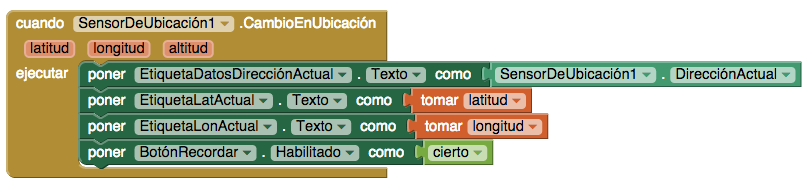
\includegraphics[scale=0.5]{Sensors2}
\caption{Utilizando el \component{SensorDeUbicación} para leer la ubicación actual.}
\label{fig:Sensors2}
\end{figure}

\paragraph{Prueba tu Aplicación!} Probar tu aplicación en vivo, es
decir probarla en un teléfono conectado a tu computador, no funciona
para las aplicaciones basadas en medición de ubicación. Tienes que
empaquetar la aplicación como archivo .apk y luego instalarla en tu
teléfono. Si no tienes lectura del GPS, revisa tus ajustes en Android,
y prueba en distintos lugares.

\subsubsection*{Registrar la ubicación actual}

Cuando el usuario presiona el \component{BotónRecordar}, los datos de
ubicación más actualizados deberían ser colocarse dentro de las
etiquetas para mostrar los datos registrados. La
Tabla~\ref{tab:Sensors4} muestra los bloques que necesitarás para esta
funcionalidad.

\begin{table}
\centering
\begin{footnotesize}
\begin{tabular}{|l|p{6cm}|}
\hline
Tipo de Bloque & Propósito\\\hline

\block{BotónRecordar.Click} & Se activa cuando el usuario presiona el
botón ``Recordar Mi Ubicación Actual''.\\\hline

\block{poner EtiquetaDatosLugarRecordado.Texto} & Coloca los datos de
dirección del sensor dentro de la etiqueta para el lugar
recordado.\\\hline

\block{SensorDeUbicación1.DirecciónActual} & Esta propiedad te da una
dirección ``de calle'' para las coordenadas leídas del GPS.\\\hline

\block{poner EtiquetaLatLugarRecordado.Texto} & Coloca la latitud
dentro de la etiqueta correspondiente al lugar recordado.\\\hline

\block{poner EtiquetaLonLugarRecordado.Texto} & Coloca la longitud
dentro de la etiqueta correspondiente al lugar recordado.\\\hline
\end{tabular}
\end{footnotesize}
\caption{Bloques para registrar y mostrar la ubicación actual.}
\label{tab:Sensors4}
\end{table}

Cuando el usuario presiona el \component{BotónRecordar}, las lecturas
actuales del sensor de ubicación son colocadas en las etiquetas
``lugar recordado'', como lo la~\Cref{fig:Sensors3}.

\begin{figure}[H]
\centering
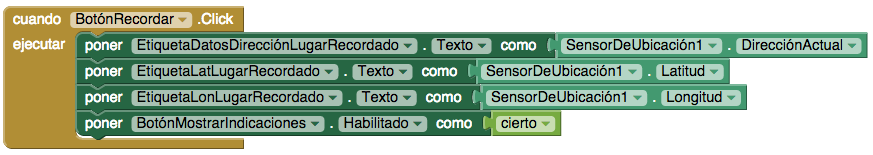
\includegraphics[scale=0.5]{Sensors3}
\caption{Colocando la información sobre la ubicación actual en las
  etiquetas ``lugar recordado''.}
\label{fig:Sensors3}
\end{figure}

Si te das cuenta, el \component{BotónMostrarIndicaciones} está
activado. Podría ser delicado, por que si el usuario hace click en el
botón inmediatamente, la ubicación registrada será la misma que la de
la ubicación actual---entonces el mapa que aparecería no daría mucha
información en términos de indicaciones. Sin embargo, esto es algo que
no debería suceder muy a menudo (y si sucede no es muy grave);
típicamente el usuario se moverá luego de almacenar la ubicación, (por
ejemplo, camina al concierto), por lo tanto la ubicación actual y la
ubicación recordada serán diferentes.

\paragraph{Prueba tu Aplicación!} Descarga la nueva versión de la
aplicación en tu teléfono y pruebala de nuevo. Cuando presionas el
\component{BotónRecordar}, ¿se copia la ubicación actual como la
ubicación recordada?

\subsubsection*{Mostrar indicaciones hacia el lugar recordado}

Cuando el usuario presiona el \component{BotónMostrarIndicaciones},
quieres que la aplicación abra Google Maps con las indicaciones desde
la ubicación actual del usuario hacia la ubicación registrada (en este
caso, donde el auto está estacionado).

El componente \component{ActivityStarter} puede abrir cualquier
aplicación Android, incluyendo Google Maps. Tienes que ajustar algunos
parámetros de configuración para poder usarlo, pero para abrir algo
como un navegador web o un mapa, los parámetros que tienes que
especificar son bastante simples.

Para abrir un mapa, la propiedad clave que tienes que configurar es
\property{ActivityStarter.UriDelDato}. En esta propiedad puedes poner
cualquier URL que pueda ser ingresada directamente en un navegador
web. Si quieres explorar este punto, abre \url{http://maps.google.cl}
en tu navegador web y pregunta por indicaciones entre Santiago y
Valparaíso. Cuando aparezcan las indicaciones, mira la barra de
direcciones. Este es el tipo de URL que tienes que construir en tu
aplicación.

La diferencia en el caso de tu aplicación es que el mapa de
indicaciones que vas a crear será desde un conjunto de coordenadas GPS
a otro conjunto de coordenadas GPS (no de ciudad a ciudad). El enlace
mencionado anteriormente es similar a este:
\url{https://www.google.com/maps/dir/Santiago/Valparaiso}. Copia este
URL en un navegador web para averiguar lo que muestra.

Para esta aplicación, necesitas construir la URL
\url{http://maps.google.com/maps/?saddr=0.1,0.1\&daddr=0.2,0.2} y
fijar sus parámetros de dirección de origen (\emph{saddr} o
\emph{source address} en inglés) y dirección de destino (\emph{daddr}
o \emph{destination address} en inglés) dinámicamente. Recuerda que
ayer concatenaste textos usando \block{unir}; haremos eso aquí
también, conectando los datos GPS para las ubicaciones registrada y
actual. Pondrás el URL que has construido en la propiedad
\component{ActivityStarter.UriDelDato}, y después llamarás a
\block{ActivityStarter.IniciarActividad}. La Tabla~\ref{tab:Sensors5}
lista todos los bloques que necesitarás para eso.

Cuando el usuario presiona el \component{BotónMostrarIndicaciones}, el
controlador de evento construye una URL para un mapa y llama a
\component{ActivityStarter} para lanzar la aplicación Google Maps y
cargar el mapa, como lo muestra la~\Cref{fig:Sensors4}. Se usa
\block{unir} para construir la URL que se envia a Google Maps.

La URL resultante consiste en el dominio de Google Maps
(\url{http://maps.google.com/maps}) con dos parametros de URL,
\emph{saddr} y \emph{daddr}, que especifican las ubicaciones de origen
y de destino para las direcciones. Para esta aplicación, \emph{saddr}
corresponde a la latitud y longitud actuales, y \emph{daddr}
corresponde a la latitud y longitud de la ubicación almacenada.

\begin{table}
\centering
\begin{tabular}{|l|p{6cm}|}
\hline
Tipo de Bloque & Propósito\\\hline

\block{BotónMostrarIndicaciones.Click} & Se activa cuando el usuario
presiona el botón ``Mostrar indicaciones...''.\\\hline

\block{poner ActivityStarter.DatoDelURI} & Fija la URL del mapa que
quieres mostrar.\\\hline

\block{unir} & Construye una URL a partir de varias partes.\\\hline

Bloque de texto ``http://maps.google.com/maps/?saddr='' & La parte
fija de la URL, que contiene el parámetro para la dirección de
origen.\\\hline

\block{EtiquetaLatActual.Texto} & La latitud actual.\\\hline

Bloque de texto ``,'' & Pone una coma entre los valores de latitud y
longitud.\\\hline

\block{EtiquetaLonActual.Texto} & La longitud actual.\\\hline

Bloque de texto ``\&addr='' & Agrega el segundo parámetro a la URL, la
ubicación de destino.\\\hline

\block{EtiquetaLatLugarRecordado} & La latitud registrada.\\\hline

Bloque de texto ``,'' & Pone una coma entre los valores de latitud y
longitud.\\\hline

\block{EtiquetaLonLugarRecordado} & La longitud registrada.\\\hline

\block{ActivityStarter.IniciarActividad} & Abre Google Maps.\\\hline  
\end{tabular}  
\caption{Bloques para registrar y mostrar la ubicación actual.}
\label{tab:Sensors5}
\end{table}

\begin{figure}[H]
\vspace{3em}
\centering
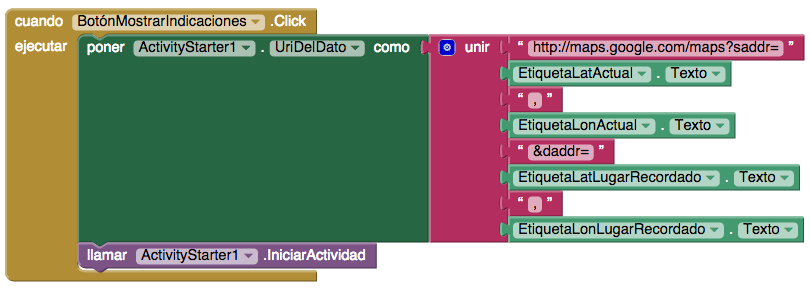
\includegraphics[scale=0.5]{Sensors4}
\caption{Construir la URL a usar para abrir Google Maps.}
\label{fig:Sensors4}
\end{figure}

\paragraph{Prueba tu Aplicación!} Descarga la nueva versión de la
aplicación en tu teléfono y pruébala de nuevo. Cuando una lectura GPS
llegue, presiona el \component{BotónRecordar} y cambia tu
ubicación. Cuando presionas el \component{BotónMostrarIndicaciones},
¿el mapa te muestra como volver a tu ubicación inicial? Después de
mirar el mapa, presiona el botón ``Volver'' un par de veces para
volver a la aplicación.

\subsubsection*{Guardar la ubicación registrada persistentemente}

Ahora tienes una aplicación que funciona completamente y que recuerda
una ubicación de inicio y muestra un mapa con indicaciones para volver
a esta ubicación desde donde se encuentra el usuario. Pero si el
usuario registra una ubicación y después cierra la aplicación, los
datos registrados no estarán disponibles cuando la abrira de nuevo.

Lo que quieres es que el usuario pueda registrar la ubicación de su
auto, cerrar la aplicación, ir a su evento, y lanzar la aplicación de
nuevo después de su evento para tener indicaciones hacia su auto.

Si ya estás pensando en la aplicación \appName{No SMS al Volante}, estás bien!
Necesitamos almacenar datos de manera persistente en una base de datos
usando \component{TinyDB}. Necesitarás un esquema similar al utilizado en la
aplicación que desarrollaste ayer:

\begin{enumerate}

\item Cuando el usuario hace click en \component{BotónRecordar},
  almacena los datos de ubicación en la base de datos.

\item Cuando la aplicación se abre, carga los datos de ubicación desde
  la base de datos dentro de una variable o propiedad.
\end{enumerate}

Empezarás modificando el controlador de evento
\block{BotónRecordar.Click} para que almacene los datos
registrados. Para guardar la latitud, longitude, y dirección,
necesitarás tres llamadas a \block{TinyDB.GuardarValor}. La
Tabla~\ref{tab:Sensors6} muestra los bloques adicionales que
necesitarás.

\begin{table}
\centering
\begin{tabular}{|l|p{6cm}|}
\hline
Tipo de Bloque & Propósito\\\hline

\component{TinyDB1.GuardarValor} & Almacena los datos en la base de
datos del equipo.\\\hline

Bloque de texto ``dirección'' & Etiqueta para usarse con
\component{TinyDB1.GuardarValor}.\\\hline

\component{SensorDeUbicación.DirecciónActual} & La dirección a
almacenar persistentemente dentro del parámetro \parameter{valor} del
bloque \block{TinyDB1.GuardarValor}.\\\hline

Bloque de texto ``lat'' & Etiqueta para usarse en
\block{GuardarValor}.\\\hline

\component{SensorDeUbicación.Latitud} & La latitud a almacenar
persistentemente, usando \block{GuardarValor}.\\\hline

Bloque de texto ``lon'' & Etiqueta para usarse en
\block{GuardarValor}.\\\hline

\component{SensorDeUbicación.Longitud} & La longitud a almacenar
persistentemente, usando \block{GuardarValor}.\\\hline  
\end{tabular}  
\caption{}
\label{tab:Sensors6}
\end{table}

Como se muestra en la~\Cref{fig:Sensors5},
\block{TinyDB1.GuardarValor} copia los datos de ubicación desde las
propiedades del \component{SensorDeUbicación} en la base de datos.

Como lo podrás recordar de la aplicación \appName{No SMS al Volante},
la función \block{GuardarValor} tiene dos argumentos, la etiqueta y el
valor. La etiqueta identifica los datos que quieres almacenar, y el
valor es el lo que quieres almacenar---en este caso los datos de del
\component{SensorDeUbicación}.

\begin{figure}[H]
\vspace{3em}
\centering
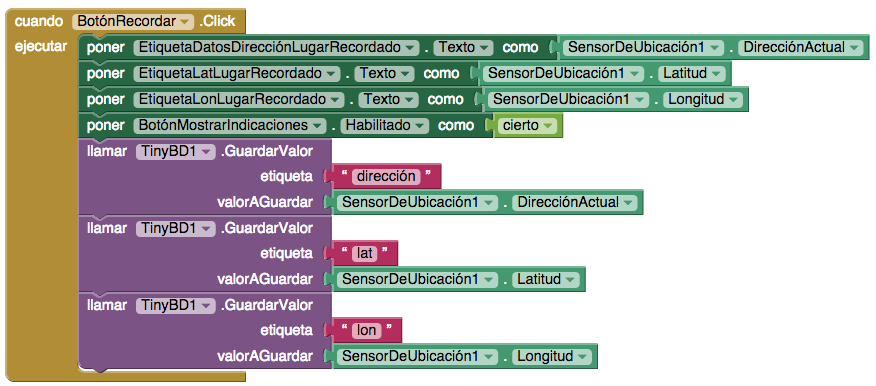
\includegraphics[scale=0.5]{Sensors5}
\caption{Almacenando los datos de ubicación en una base de datos.}
\label{fig:Sensors5}
\end{figure}

\subsubsection*{Recuperar la ubicación registrada cuando la aplicación se lanza}

Almacenas datos en una base de datos para que puedas acceder a estos
datos en el futuro. En este aplicación, si un usuario almacena una
ubicación y después cierra la aplicación, quieres recuperar esta
información desde la base de datos y mostrarla al usuario cuando
lanzará la aplicación de nuevo.

Como se vio en los días anteriores, el evento
\component{Screen.Inicializar} se activa cuando tu aplicación se
abre. Recuperar datos desde una base de datos es una cosa muy común de
hacer cuando se abre la aplicación, y es exactamente lo que queremos
hacer en el caso de esta aplicación.

Usarás la función \block{TinyDB.ObtenerValor} para recuperar los datos
GPS almacenados. Como necesitas recuperar la dirección, latitud, y
longitud almacenadas, necesitarás 3 llamadas a \block{GetValue}. Como
lo hicimos para \appName{No SMS al Volante}, necesitarás averiguar si
hay datos almacenados ahí o no (si es la primera vez que la aplicación
se abre, \block{TinyDB.ObtenerValor} devolverá un texto vacío).

Como desafío, ve si puedes crear estos bloques y compara tu creación
con el código que se muestra en la~\Cref{fig:Sensors6}.

\begin{figure}[H]
\vspace{3em}
\centering
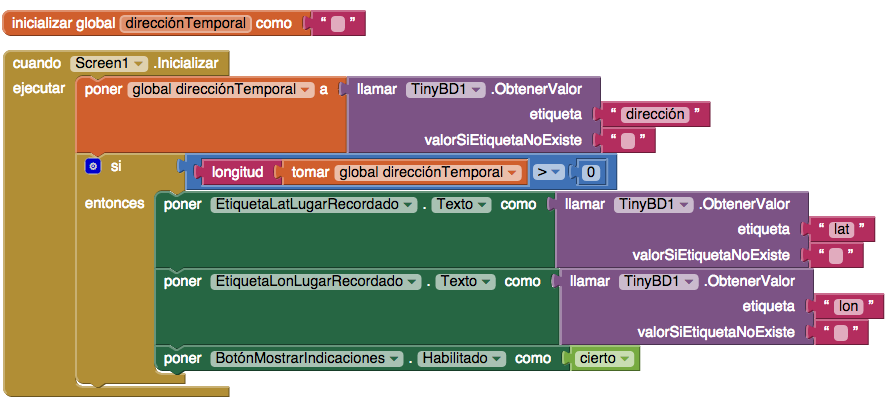
\includegraphics[scale=0.5]{Sensors6}
\caption{Añadiendo la ubicación registrada a una base de datos para
  que esté disponible cuando la aplicación se cierra y se abre de
  nuevo.}
\label{fig:Sensors6}
\end{figure}

Para entender estos bloques, puedes visualizar a un usuario abriendo
la aplicación por la primera vez, y abriendola más tarde después de
haber registrado los datos de ubicación. La primera vez que el usuario
abre la aplicación, no habrá datos de ubicación en la base de datos
por cargar, entonces no quieres fijas las etiquetas ``lugar
recordado'' o activar el \component{BotónMostrarIndicaciones}. Al
abrir la aplicación sucesivamente, si hay datos almacenados, lo que
quieres es cargar los datos de ubicación almacenados previamente desde
la base de datos.

Estos bloques primero llaman a \block{TinyDB1.ObtenerValor} con una
etiqueta ``dirección'', una de las etiquetas utilizadas cuando
guardaste los datos de ubicación más temprano. El valor recuperado se
coloca en una variable \variable{direcciónTemporal}, donde se averigua
si está vacío o contiene datos.

El bloque condicional es necesario porque \component{TinyDB} devuelve
texto vacío si no hay datos para una etiqueta dada; no hay ningún
datos la primera vez que la aplicación está lanzada y no habrá hasta
que el usuario presione el \component{BotónRecordar}. Dado que ahora
la variable \variable{direcciónTemporal} tiene el valor devuelto,
debes averiguar si el largo de \variable{direcciónTemporal} es
superior a 0. Si el largo es superior a 0, la aplicación sabe que
\component{TinyDB} devolvió algo, y el valor recuperado es colocado en
\component{EtiquetaDatosLugarRecordado}. La aplicación también sabe
que si una dirección ha sido almacenada, tiene una latitud y una
longitud. Entonces, estos valores también son recuperados usando
\block{TinyDB.ObtenerValor}. Finalmente, si datos ha sido recuperados,
se activa el \component{BotónMostrarIndicaciones}.

\paragraph{Prueba tu Aplicación!} Descarga la nueva versión de tu
aplicación en tu teléfono y pruebala de nuevo. Presiona el
\component{BotónRecordar} y asegúrate que las lecturas están
registradas. Luego cierra la aplicación y abrela de nuevo. ¿Los datos
registrados aparecen?

\subsection*{Resumen}

Aquí van algunos de los conceptos que vimos en este tutorial:

\begin{itemize}

\item El componente \component{SensorDeUbicación} reporta la latitud,
  longitud, altitud, y dirección actuales del usuario. El evento
  \block{CambioDeUbicación} se activa cuando el sensor obtiene su
  primera lectura y cuando la lectura cambia (o sea, cuando el equipo
  se movió).

\item El componente \component{ActivityStarter} puede lanzar cualquier
  aplicación, incluyendo Google Maps. Para Google Maps, fijas la
  propiedad \property{UriDelDato} con la URL del mapa que quieres
  mostrar. Si quieres mostrar indicaciones entre coordenadas GPS, la
  URL será en el formato siguiente, pero reemplazando los datos del
  ejemplo con coordenadas GPS reales:
  \url{http://maps.google.com/maps/?saddr=0.1,0.1\&daddr=0.2,0.2}.

\item El bloque \block{unir} se utiliza para concatenar (juntar)
  elementos de texto separados dentro de un sólo objeto de
  texto. Permite concatenar datos dinámicos con texto estático. Con la
  URL para Google Maps, las coordenadas GPS son datos dinámicos.

\item \component{TinyDB} te permite almacenar datos de manera
  persistente en la bases de datos del teléfono. Los datos almacenados
  en una base de datos pueden ser cargados cada vez que la aplicación
  se abre.
\end{itemize}

\section{Material de Apoyo}

\subsection*{Geolocalización}

Los dispositivos de geolocalización, o más conocidos como GPS, se
comunican con una serie de satélites y otros mecanismos para
determinar la ubicación de tu teléfono o tablet. La pregunta esencial
que responden estos sensores es: ``¿Dónde estoy?''

\paragraph{Ejemplo: ¿Cómo muestras tu latitud, longitud y dirección
  actual?}

El evento \block{SensorDeUbicación.CambioEnUbicación} se activa:

\begin{enumerate}

\item la primera vez la aplicación obtiene una lectura desde los
  satélites GPS u otros mecanismos.

\item cuando la ubicación del dispositivo cambia. Si estás caminando,
  podría activarse varias veces.

\end{enumerate}

Nota que puedes controlar la frecuencia de activación de
\block{CambioEnUbicación} con las propiedades
\property{SensorDeUbicación.IntervaloDeTemporizador} y
\property{SensorDeUbicación.IntervaloDeDistancia}. Por defecto, el
\property{IntervaloDeTemporizador} tiene valor de 60.000 milisegundos,
(1 minuto). Eso quiere decir que \block{CambioEnUbicación} será
activado de nuevo solamente después de un minuto.

En el ejemplo de la~\Cref{fig:Geo1}, las lecturas de ubicación se
muestran en etiquetas. La latitud y longitud son números, mientras que
la propiedad \property{DirecciónActual} provee una dirección (con
calle, avenida, etc.) para la ubicación actual. Si caminas verás que
los números y la dirección cambian.

\begin{figure}[H]
  \centering
  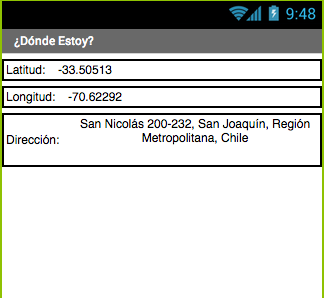
\includegraphics[scale=0.5]{Geo1}
  \caption{Mostrando la latitud, longitud, y dirección actuales.}
  \label{fig:Geo1}
\end{figure}

\paragraph{Ejemplo: ¿Cómo sabes lo lejos que estás de un punto dado?}

\AppInventor no provee un bloque ``distancia'' para calcular la
distancia entre dos coordenadas GPS. Pero existen fórmulas matemáticas
conocidas para aproximar la distancia entre dos puntos. La solución
consiste en crear tu propio block---un procedimiento--- y conectarlo a
las fórmulas conocidas. Una vez que tienes la el procedimiento para la
distancia, puedes llamarla al final del controlador de evento
\block{CambioDeUbicación}. El ejemplo de la~\Cref{fig:Geo2} muestra
cómo se calcula la distancia entre el punto actual y las oficinas de
Inria Chile.

\begin{figure}[H]
  \centering
  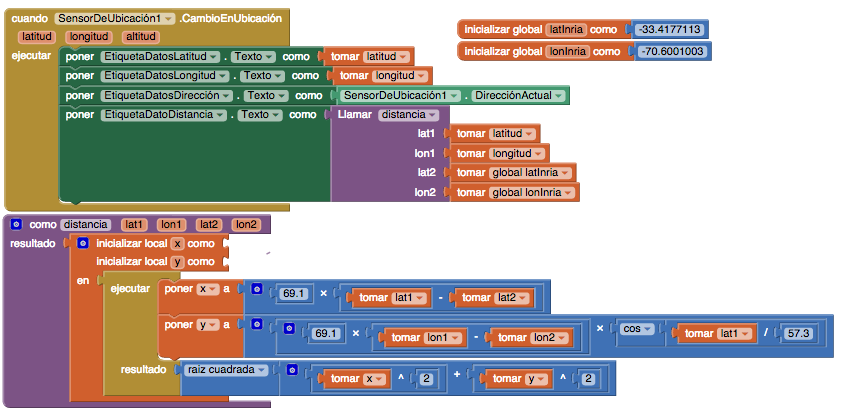
\includegraphics[scale=0.5]{Geo2}
  \caption{Calculando la distancia entre dos coordenadas GPS.}
  \label{fig:Geo2}
\end{figure}

El procedimiento \procedure{distancia} es un poco más sofisticado que
los que hemos visto hasta ahora: posee 4 parámetros, y además devuelve
un valor como resultado. Veremos esto en más detalle en el Día 7 del
taller.


\subsubsection*{Creando aplicaciones basadas en la ubicación}

Hasta la popularización de los smartphones, la computación estaba
limitada a los computadores de escritorio. Bueno, los laptops son
móviles, pero no en el mismo sentido que los pequeños equipos que
podemos poner en nuestros bolsillos. La computación ha dejado las
oficinas y los laboratorios y se está moviendo afuera en todo el
mundo.

Un efecto significante de llevar nuestro equipo de computación con
nosotros es poder utilizar un dato nuevo y muy interesante: la
ubicación actual. Saber dónde se encuentra la gente mientras se está
moviendo en el mundo tiene grandes implicaciones y el potencial de
ayudarnos en nuestras vidas.  También tiene el potencial de invadir
nuestra privacidad y ser un detrimento de la humanidad.

La aplicación \appName{¿Dónde está mi Auto?} es un ejemplo de una
aplicación basada en la ubicación que trae un beneficio personal. Esta
aplicación es privada, la información de tu ubicación está almacenada
únicamente en la base de datos de tu teléfono.

La medición de ubicación puede también ser utilizada por grupos. Por
ejemplo, un grupo de personas que está haciendo trekking podría querer
seguir los movimientos de los otros en la montaña, o colegas de
trabajos podrían querer poder encontrarse en una gran conferencia.
Algunas personas utilizan este tipo de aplicación ``check-in'' todos
los días.

Otro tipo de aplicación basada en la ubicación utiliza herramientas de
\emph{realidad aumentada}. Estas aplicaciones utilizan tu ubicación y
la orientación de tu teléfono para proveer información extra que
aumenta los ajustes naturales. Podrías apuntar tu teléfono hacia un
edificio y ver el precio del mercado inmobiliario, o podrías caminar
cerca de una planta exótica en un jardín y ver cuál especie es con
alguna aplicación.

\paragraph{GPS}

Para crear aplicaciones basadas en la ubicación, primero tienes que
entender como el GPS (\emph{Global Positioning System} en inglés, o
\emph{Sistema de Posicionamiento Global}) funciona. Los datos GPS
vienen de un sistema de satélites mantenido por el gobierno
estadounidense. Siempre y cuando existe una vista despejada de al
menos 3 satélites en el sistema, tu teléfono puede obtener una
lectura. Una lectura GPS consiste en tu latitud, longitud y
altitud. Latitud es cuán lejos de la línea del Ecuador hacia el norte
o el sur te encuentras, con valores positivos hacia el norte y
negativos hacia el sur. La gama de valores es de -90 a
90. La~\Cref{fig:Geo3} muestra un mapa Google de un lugar cerca de
Quito, capital del Ecuador. La latitud mostrada en el mapa es 0.08,
apenas al norte de la línea del Ecuador.

\begin{figure}[H]
  \centering
  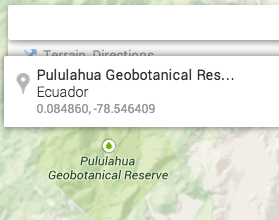
\includegraphics[scale=0.5]{Geo3}
  \caption{Un lugar muy cercano a la línea del Ecuador.}
  \label{fig:Geo3}
\end{figure}

La longitud es cuán lejos del primer meridiano hacia el este u oeste
te encuentras, con valores positivos hacia el este y negativos hacia
el oeste. El lugar más conocido por el cual pasa el meridiano es
Greenwich, una ciudad cerca de Londres, casa del Observatorio Real. El
mapa de la~\Cref{fig:Geo4} muestra Greenwich y su longitud es muy
cercana a $0.0$.

\begin{figure}[H]
  \centering
  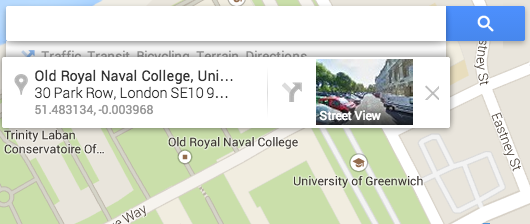
\includegraphics[scale=0.5]{Geo4}
  \caption{Un lugar muy cercano al meridiano de Greenwich.}
  \label{fig:Geo4}
\end{figure}

\paragraph{Medir la ubicación con \AppInventor}

\AppInventor viene con el componente \component{SensorDeUbicación}
para acceder a información del GPS. El componente tiene propiedades
para la \property{Latitud}, \property{Longitud}, y
\property{Altitud}. También secomunica con Google Maps, para que
puedas tener una lectura para tu dirección actual.

El evento \block{SensorDeUbicación.CambioEnUbicación}, mostrado en
la~\Cref{fig:Geo5}, es el controlador de evento más importante del
\component{SensorDeUbicación}.

\begin{figure}[H]
  \centering
  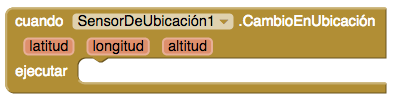
\includegraphics[scale=0.5]{Geo5}
  \caption{Un lugar muy cercano al meridiano de Greenwich.}
  \label{fig:Geo5}
\end{figure}

Este evento se activa la primera vez que el sensor tiene una lectura y
cada vez que el teléfono se mueve lo suficiente como para que una
nueva ubicación pueda ser leída. Es frecuente tener una demora de
algunos segundos antes de la primera lectura de una aplicación, y a
veces el equipo no puede obtener lectura. Por ejemplo, si estás en una
pieza cerrada y sin conexión WiFi, podría ser que el equipo no obtenga
una lectura. Tu telefono tambien tiene ajustes que te permiten apagar
la lectura GPS para ahorrar batería; es otra potencial razón por la
cual el equipo podría no obtener lectura.

Por estas razones, no tienes que suponer que las propiedades del
\component{SensorDeUbicación} tienen valores válidos hasta que se
active el evento \block{CambioEnUbicación}.

Una manera de manejar lo desconocido en la medición de ubicación es crear
una variable \variable{ultimaUbicaciónConocida}, inicializarl como
``desconocida'' y después hacer que el controlador de evento cambie el valor
de la variable, como lo muestra la~\Cref{fig:Geo6}.

\begin{figure}[H]
  \centering
  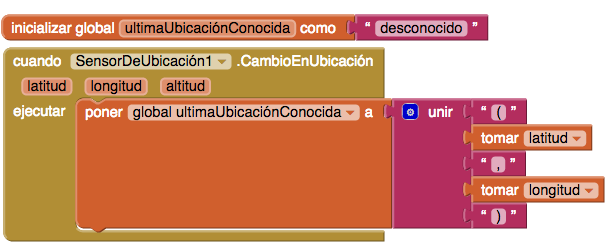
\includegraphics[scale=0.5]{Geo6}
  \caption{El valor de la variable \variable{ultimaUbicaciónConocida}
    cambia junto con el cambio de ubicación.}
  \label{fig:Geo6}
\end{figure}

Programando el controlador de evento
\block{SensorDeUbicación.CambioEnUbicación} de esta manera, siempre
  podrás mostrar la ubicación actual o registrarla en una base de
  datos, con ``desconocido'' apareciendo hasta la primera lectura.

También puedes preguntar explícitamente si el sensor tiene una lectura
utilizando el bloque \block{SensorDeUbicación.TieneLongitudYAltitud},
como se muestra en la~\Cref{fig:Geo7}.

\begin{figure}[H]
  \centering
  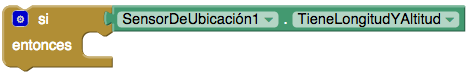
\includegraphics[scale=0.5]{Geo7}
  \caption{Probando si el sensor tiene una lectura con el bloque \block{TieneLongitudYAltitud}.}
  \label{fig:Geo7}
\end{figure}

\paragraph{Averiguando los límites}

Un uso común del evento \block{CambioEnUbicación} es de averiguar si
el equipo se encuentra dentro de una zona geográfica. Por ejemplo,
considera el código de la~\Cref{fig:Geo8}, que hace vibrar el teléfono
cada vez que una nueva lectura muestra que el usuario se ha movido más
lejos que 0.1 de longitud desde el primer meridiano.

\begin{figure}[H]
  \centering
  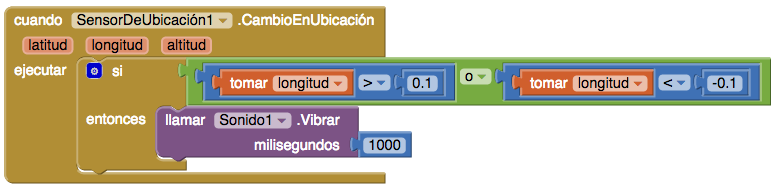
\includegraphics[scale=0.5]{Geo8}
  \caption{Si una lectura no está cerca del primer meridiano, el
    teléfono vibra.}
  \label{fig:Geo8}
\end{figure}

Tal revisión de límites (zona límite, o \emph{geocercas}) tiene varias aplicaciones; por
ejemplo alertar personas en libertad condicional si se encuentran a una
distancia superior de su casa que la distancia límite, o alertar padres
o profesores si un niño se mueve fuera del parque infantil.

\paragraph{Proveedores de información de ubicación: GPS, WiFi, y Cell ID}

Un equipo Android puede determinar su ubicación de varias maneras. El
método más preciso---dentro de algunos metros---es a través de los
satélites GPS. Sin embargo, no tendrás lectura si te encuentras en un
edificio y si hay rascacielos u otros objetos entre ti y los
satélites; necesitas poder acceder al menos a 3 satélites del sistema.

Si el GPS no está disponible o el usuario lo ha desactivado, el equipo
puede obtener su ubicación a través de una red inalámbrica.  Tienes
que estar cerca de un router WiFi y la lectura de ubicación que
obtendrás será la latitude y longitude del router WiFi.

Una tercera manera con la cual un equipo puede determinar su ubicación
es a través de Cell ID. Cell ID provee una ubicación para el telefono,
basada en la fuerza de los señales de las torres celulares cerca del
usuario. En general este método no es muy preciso, excepto si tienes
varias torres celulares cerca de ti. Sin embargo, utiliza una mínima
cantidad de batería comparado a los métodos basados en GPS y WiFi.

\subsection*{Otros Sensores}

Los dispositivos Android poseen una variedad de sensores en adición al
\component{Acelerómetro} y el \component{SensorDeUbicación} que ya
hemos visto en algunas aplicaciones. Ahora veremos cómo usar el
\component{SensorDeOrientación} y exploraremos un poco más en
profundidad las capacidades del acelerómetro.


\subsubsection*{Utilizar el Sensor de Orientación}

El \component{SensorDeOrientación} es utilizado en juegos en los
cuales el usuario controla las acciones inclinando el equipo. También
puede ser utilizado en una aplicación como una brújula, para encontrar
hacia qué dirección (norte/sur, este/oeste) el teléfono está
apuntando.

% Angulo - Angle
% Acimut - Azimuth
% Magnitud - Magnitud
% Tono - Pitch
% Lanzar - Roll

El \component{SensorDeOrientación} tiene cinco propiedades, todas
desconocidas de la mayoría de las personas, excepto los ingenieros
aeronáuticos:

\begin{itemize}
\item \property{Lanzar} (Izquierda--Derecha): Lanzar es de 0 grados
  cuando el equipo está nivelado, aumenta a 90 grados cuando el equipo
  está inclinado hacia la izquierda, y disminuye a -90 grados cuando
  el equipo está inclinado hacia la derecha.

\item \property{Tono}: Tono es de 0 grados cuando el equipo está
  nivelado, aumenta a 90 grados cuando el equipo está inclinado de tal
  manera que la parte superior apunta abajo, y aumenta a 180 grados
  cuando el equipo está dado vuelta.

  De manera similar, cuando el equipo está inclinado de tal manera que
  la parte abajo apunta abajo, Pitch disminuye a -90 grados y a -180
  grados si está dado vuelta enteramente.

\item \property{Acimut} (Compás): Acimut es de 0 grados cuando el
  equipo apunta hacia el norte, 90 grados cuando apunta al este, 180
  cuando apunta al sur y 270 grados cuando apunta al oeste.

\item \property{Magnitud}: Magnitud devuelve un número entre 0 y 1 que
  indica cuanto el equipo está inclinado. Su valor indica la fuerza
  ejercida por una pelota en la superficie del equipo.

\item \property{Ángulo}: Ángulo la dirección hacia la cual el equipo
  está inclinado. Es decir, la dirección de la fuerza que ejercería
  una pelota rotando en la superficie del equipo.

\end{itemize}

El \component{SensorDeOrientación} provee el evento\block{CambioEnOrientación}, que se
activa cada vez que la orientación cambia. Para explorar estas
propiedades, escribe una aplicación que ilustra cómo las propiedades
cambian con la inclinación del equipo. Solamente añade cinco etiqueta de
título y cinco otras para mostrar los valores actuales de las
propiedades que acabamos de ver. Después añade los bloques mostrados
en la~\Cref{fig:OtherSensors1}.

\begin{figure}[H]
\centering
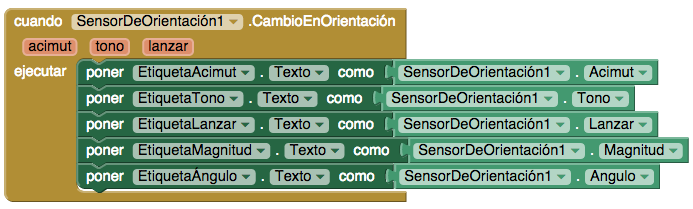
\includegraphics[scale=0.5]{OtherSensors1}
\caption{Bloques para mostrar los datos del \component{SensorDeOrientación}.}
\label{fig:OtherSensors1}
\end{figure}

\subsubsection*{Utilizar el parámetro Lanzar para mover un objeto}

Ahora vamos a tratar de mover una imagen a la izquierda o a la derecha
inclinando el equipo, como ocurre en algunos juegos de
autos. Selecciona un \component{Lienzo} y ajusta el ancho a ``Ajustar
al contenedor'' y el alto a 200 pixeles. Luego añade
\component{SpriteImagen} o una \component{Pelota} dentro del lienzo, y
añade una etiqueta, \component{EtiquetaLanzar}, para desplegar un
valor de propiedad, como lo muestra la~\Cref{fig:OtherSensors2}.

\begin{figure}[H]
\centering
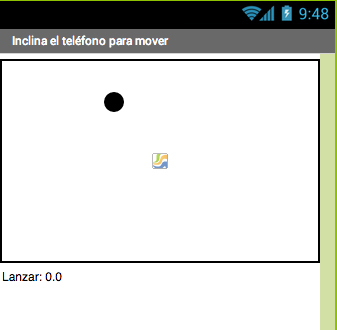
\includegraphics[scale=0.5]{OtherSensors2}
\caption{Una interfaz de usuario para explorar como el sensor de
  ubicación puede utilizarse para mover una imagen.}
\label{fig:OtherSensors2}
\end{figure}

La propiedad \property{Lanzar} del sensor de orientación te dirá si el
teléfono está inclinado a la izquierda o a la derecha (es decir, si
pones el telefono derecho y lo inclinas un poco hacia la izquierda
tendrás una lectura positiva para \property{Lanzar}; si lo inclinas un
poco hacia la derecha, tendrás una lectura negativa).

De esta manera, puedes dejar el usuario mover un objeto con el
gestionador de evento como el mostrado en la~\Cref{fig:OtherSensors2}.

\begin{figure}[H]
\centering
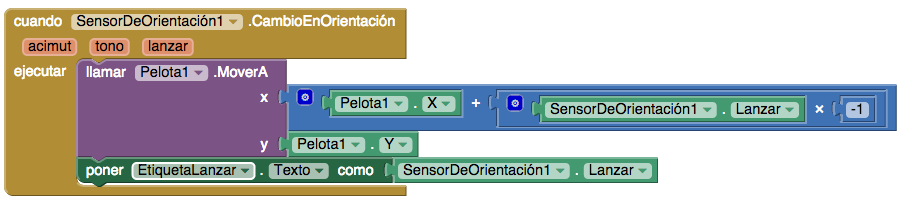
\includegraphics[scale=0.5]{OtherSensors3}
\caption{Contestando a los cambios en la propiedad \property{Lanzar}
  con el evento \block{CambioEnOrientación}.}
\label{fig:OtherSensors3}
\end{figure}

En el código hay que multiplicar el valor de \property{Lanzar} $-1$,
porque la inclinación a la izquierda da un valor positivo, pero se
debe mover el objeto disminuyendo la coordenada X.

\textbf{Importante}: esta aplicación funciona solamente cuando el
equipo está en modo \emph{retrato} (\emph{portrait} en inglés), y no
en modo \emph{paisaje}. Si inclinas el teléfono demasiado, la pantalla
cambiará al modo paisaje y la imagen se quedará al lado izquierdo de
la pantalla. La razón es que si el equipo está totalmente de lado,
está inclinado a la izquierda y entonces siempre tendrá una lectura
positiva para \property{Lanzar}. Una lectura positiva para
\property{Lanzar}, como lo muestra la~\Cref{fig:OtherSensors3} siempre
hará que la coordenada X tenga un valor más pequeño.

Nota que \AppInventor provee la propiedad
\property{Screen.OrientaciónDeLaPantalla} que puede ser utilizada para
bloquear la orientación si no quieres que cambie de modo.

\subsubsection*{Movimiento en cualquier dirección usando \property{Dirección} y \property{Magnitud}}

En el ejemplo anterior, usamos los sensores para mover la imagen a la
izquierda o a la derecha. Si quieres que el movimiento pueda tener
lugar en cualquier dirección, debes usar las propiedades
\property{Ángulo} y \property{Magnitud} del
\component{SensorDeOrientación}.

En la~\Cref{fig:OtherSensors4}, puedes ver los bloques para una
aplicación que deja al usuario inclinar el equipo para mover un sprite
en cualquier dirección (necesitas dos etiquetas y una imagen para este
ejemplo).

\begin{figure}[H]
\centering
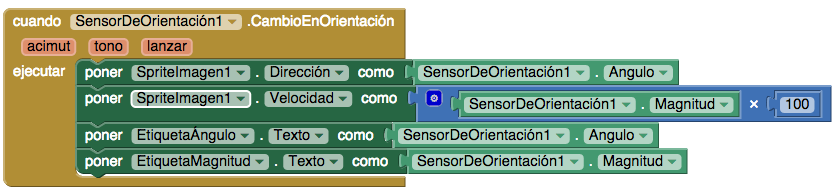
\includegraphics[scale=0.5]{OtherSensors4}
\caption{Moviendo un sprite utilizando el ángulo y la magnitud del
  sensor de orientación.}
\label{fig:OtherSensors4}
\end{figure}

\paragraph{Pruébalo!}

La propiedad \property{Magnitude}, que es un valor entre 0 y 1, denota
cuán inclinado está el equipo. En el código anterior, el sprite se
mueve más rápido mientras mayor sea la magnitud.

\subsubsection*{Usar el teléfono como una brújula}

Las aplicaciones de brújula y aplicaciones como Google Sky Map
necesitan saber la orientación del teléfono en el mundo, este/oeste y
norte/sur.  Sky Map utiliza la información para añadir información
sobre las constelaciones hacia las cuales el teléfono está apuntando.

La lectura del \property{Acimut} útil para este tipo de
orientación. \property{Acimut} siempre está entre 0 y 360 grados, 0 es
el norte; 90, este; 180, sur; and 270, oeste. Entonces, una lectura de
45 grados quiere decir que el teléfono está apuntando al noreste, 135
quiere decir sureste, 225 suroeste and 315 norte oeste.

Los bloques de la~\Cref{fig:OtherSensors5} son para una brújula simple
que muestra un texto correspondiendo a la dirección hacia la cual el
teléfono está apuntando (e.g., Noroeste). Como lo has seguramente
notado, los bloques sólo muestran una de 4 posibilidades: noreste,
sureste, suroeste, noroeste.

\paragraph{Desafío:} ve si puedes modificar el código para mostrar
solamente una dirección (norte, sur, este, oeste) si la lectura indica
que estás apuntando dentro de algunos grados hacia ella.

\begin{figure}[H]
\centering
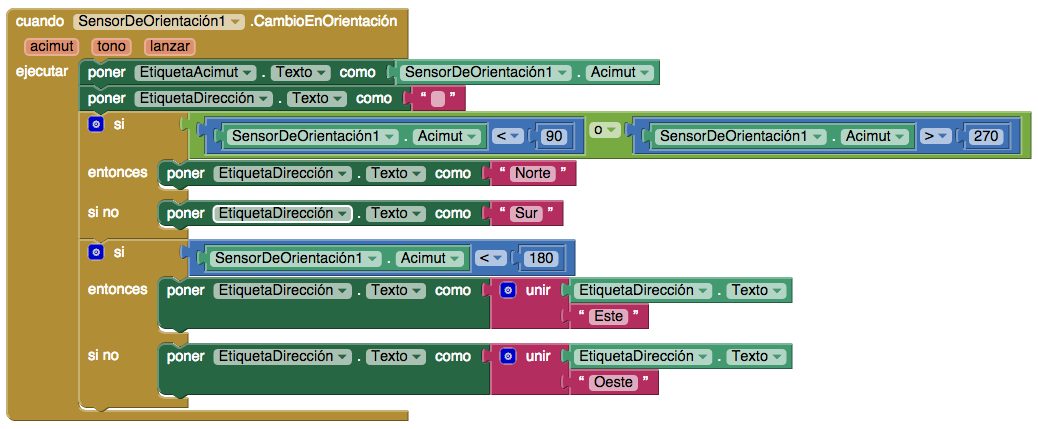
\includegraphics[scale=0.5]{OtherSensors5}
\caption{Programar una brújula simple.}
\label{fig:OtherSensors5}
\end{figure}

\subsubsection*{Utilizar el Acelerómetro}

La \emph{aceleración} es el cambio de velocidad a través del
tiempo. Si apoyas tu pie en el pedal de aceleración de un auto, el
auto acelera---su velocidad aumenta a una tasa particular.

Un acelerómetro como el que está en tu equipo Android mide la
aceleración, pero su marco de referencia no es el equipo en sí mismo,
sino que el equipo en caida libre: si haces caer el equipo, registrará
una lectura de aceleración de 0. En palabras simples, las lecturas
toman la gravedad en cuenta.

Si quieres saber más sobre los aspectos físicos, tendrás que leer
libros relacionados a Einstein o Newton! :-) Pero ahora exploraremos
el acelerometro lo suficiente para que entiendas. Vamos a examinar una
aplicación que puede salvar vidas!

\subsubsection*{Contestando a una agitación del equipo}

Ya utilizaste el sensor de aceleración durante el primer día, con el
componente \component{Acelerómetro} y el evento
\block{Acelerómetro.Agitar} para que el gatito maulle cuando se agita
el teléfono (\Cref{fig:OtherSensors6}.

\begin{figure}[H]
\centering
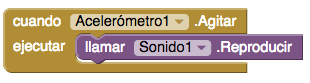
\includegraphics[scale=0.5]{OtherSensors6}
\caption{Reproducir un sonido cuando se agita el teléfono.}
\label{fig:OtherSensors6}
\end{figure}

\subsubsection*{Utilizar las lecturas del \component{Acelerómetro}}

Como los otros sensores, el acelerómetro tiene un evento para cuando
las lecturas cambian: \block{Acelerómetro.CambioEnAcceleración}. Este
evento tiene 3 argumentos que corresponden a la aceleración en 3
dimensiones:

\begin{itemize}

\item \parameter{xAccel}: Positivo cuando el equipo está inclinado a
  la derecha (es decir, su lado izquierdo está levantado), y negativo
  cuando está inclinado a la izquierda (su lado derecho está
  levantado).

\item \parameter{yAccel}: Positivo cuando la parte baja del equipo está levantada, negativo
cuando la parte alta está levantada.

\item \parameter{zAccel}: Positivo cuando la pantalla está arriba,
    negativo cuando la pantalla está mirando hacia abajo.

\end{itemize}

\subsubsection*{Detectar una caída libre}

Sabemos que si las lecturas de aceleración son cerca de 0, el equipo
está en caída libre hacia el suelo. Sabiendo eso, podemos detectar un
evento de caída libre averiguando las lecturas en el evento
\block{Acelerómetro.CambioEnAcceleración}. Estos blocks, luego de
varias pruebas, podrían ser utilizados para detectar cuando una
persona de tercera edad se ha caído y así automáticamente enviar un
mensaje de texto.

La~\Cref{fig:OtherSensors7} muestra los bloques de una aplicación que
simplemente reporta que una caída libre ocurrió (y deja el usuario
hacer click en un botón ``Reinicializar'' para averiguar de nuevo).

\begin{figure}[H]
\centering
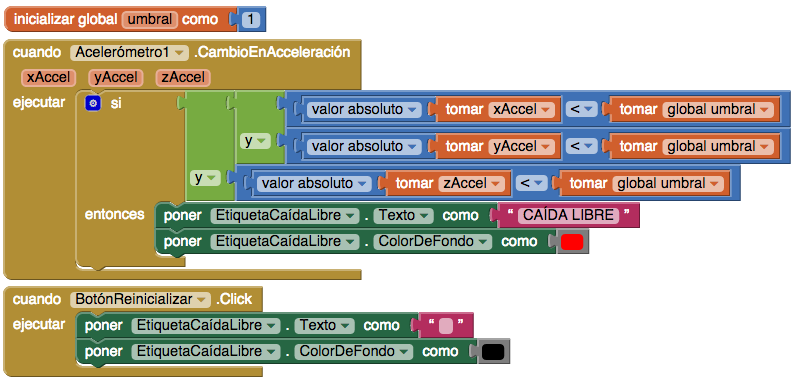
\includegraphics[scale=0.5]{OtherSensors7}
\caption{Reportar una caída libre.}
\label{fig:OtherSensors7}
\end{figure}

Cada vez que el sensor tiene una lectura, el código averigua las
dimensiones $x$, $y$, $z$ para ver si están cerca de 0 (si su valor
absoluto es inferior a 1). Si todos los tres están cerca de 0, la
aplicación cambia el texto de una etiqueta para indicar que el
teléfono está en caida. Cuando el usuario hace click en el botón
\component{BotónReinicializar}, la etiqueta vuelve a su valor
original.

\subsubsection*{Resumen}

Los sensores son de mucho interés en las aplicaciones móviles porque
permiten a los usuarios interactuar con su ambiente. Llevando el
contexto móvil a la computación, se abre un nuevo mundo de
oportunidades en experiencias de usuario y desarrollo de
aplicaciones. Sin embargo, necesitarás pensar cuidadosamente cómo,
dónde, y cuando utilizas los sensores en tus aplicaciones. Varias
personas están preocupadas por su privacidad, y podrían no usar tu
aplicación si están preocupadas de lo que estás haciendo con sus datos
de sensores. Pero con todas las opciones en los juegos, redes
sociales, viajes, y más, las posibilidades de implementar aplicaciones
positivas son casi ilimitadas.

\section{Preguntas y Personalización}

\paragraph{Preguntas}

\begin{enumerate}

\item ¿Qué quiere decir GPS, quién lo desarrolló, y de dónde vienen
  los datos?

\item ¿Qué es la latitud? ¿Qué es la longitud? Nombra un lugar con
  latitud 0, y otro lugar con longitud 0.

\item En una aplicación \AppInventor ¿cuándo se dispara el evento
  \block{SensorDeUbicación.CambioDeUbicación}? Si el evento nunca se
  dispara, ¿cuál podría ser el problema?

\item ¿Son los satélites GPS el único lugar desde el cual la
  información de ubicación proviene?

\item En una URL como la que usaste para Google Maps, ¿qué quiere
  decir ``\&''?

\item Determina la URL de Google Maps que muestra las indicaciones
  para ir desde tu casa hasta el lugar de este taller.

\item Haz un esquema de los bloques para una aplicación que manda de
  manera periódica un mensaje de texto que contiene la dirección
  actual de un equipo (dirección con calle) a un número de
  teléfono. La aplicación debería mandar un mensaje de texto cuando
  tiene una nueva lectura GPS, pero no debería mandarla más
  frecuentemente que cada 1 minuto (Pista: mira las propiedades del
  \component{SensorDeUbicación} para restringir el número de
  lecturas).

\end{enumerate}

\paragraph{Ejercicios de Personalización}


\begin{enumerate}

\item Añade información de ubicación a la aplicación \appName{No SMS
    al Volante}; es decir, cuando llega un mensaje de texto, manda el
  mensaje de texto personalizado de vuelta al remitente, pero además
  agrega la dirección actual a la respuesta.

\item Crea la aplicación \appName{¿Dónde está todo el mundo?}, una aplicación que deja
  a un grupo de persona seguir los movimientos de cada uno de sus
  miembros. Ya sea que estés subiendo una montaña o en el parque, esta
  aplicación podría ayudar a ahorrar tiempo y posiblemente vidas
  incluso. Los datos para esta aplicación están compartidos, entonces
necesitarás usar una base de datos web y el componente
\component{MiniWebDB} en vez de \component{TinyDB}. Consulta con tu
tutor para más información.

\item Crea una aplicación \appName{Migas de Pan} que sigue tus
  movimientos registrando cada cambio de ubicación en una lista. Debes
  registrar una nueva miga de pan (nueva ubicación) solamente si la
  ubicación ha cambiado de cierta forma, o solamente si una cierta
  cantidad de tiempo ha pasado, porque incluso movimientos leves
  pueden generar una nueva lectura de ubicación. Necesitarás almacenar
  las ubicaciones registradas en una lista.

\end{enumerate}